% Options for packages loaded elsewhere
\PassOptionsToPackage{unicode}{hyperref}
\PassOptionsToPackage{hyphens}{url}
\documentclass[
]{article}
\usepackage{xcolor}
\usepackage{amsmath,amssymb}
\setcounter{secnumdepth}{-\maxdimen} % remove section numbering
\usepackage{iftex}
\ifPDFTeX
  \usepackage[T1]{fontenc}
  \usepackage[utf8]{inputenc}
  \usepackage{textcomp} % provide euro and other symbols
\else % if luatex or xetex
  \usepackage{unicode-math} % this also loads fontspec
  \defaultfontfeatures{Scale=MatchLowercase}
  \defaultfontfeatures[\rmfamily]{Ligatures=TeX,Scale=1}
\fi
\usepackage{lmodern}
\ifPDFTeX\else
  % xetex/luatex font selection
\fi
% Use upquote if available, for straight quotes in verbatim environments
\IfFileExists{upquote.sty}{\usepackage{upquote}}{}
\IfFileExists{microtype.sty}{% use microtype if available
  \usepackage[]{microtype}
  \UseMicrotypeSet[protrusion]{basicmath} % disable protrusion for tt fonts
}{}
\makeatletter
\@ifundefined{KOMAClassName}{% if non-KOMA class
  \IfFileExists{parskip.sty}{%
    \usepackage{parskip}
  }{% else
    \setlength{\parindent}{0pt}
    \setlength{\parskip}{6pt plus 2pt minus 1pt}}
}{% if KOMA class
  \KOMAoptions{parskip=half}}
\makeatother
\usepackage{longtable,booktabs,array}
\newcounter{none} % for unnumbered tables
\usepackage{calc} % for calculating minipage widths
% Correct order of tables after \paragraph or \subparagraph
\usepackage{etoolbox}
\makeatletter
\patchcmd\longtable{\par}{\if@noskipsec\mbox{}\fi\par}{}{}
\makeatother
% Allow footnotes in longtable head/foot
\IfFileExists{footnotehyper.sty}{\usepackage{footnotehyper}}{\usepackage{footnote}}
\makesavenoteenv{longtable}
\usepackage{graphicx}
\makeatletter
\newsavebox\pandoc@box
\newcommand*\pandocbounded[1]{% scales image to fit in text height/width
  \sbox\pandoc@box{#1}%
  \Gscale@div\@tempa{\textheight}{\dimexpr\ht\pandoc@box+\dp\pandoc@box\relax}%
  \Gscale@div\@tempb{\linewidth}{\wd\pandoc@box}%
  \ifdim\@tempb\p@<\@tempa\p@\let\@tempa\@tempb\fi% select the smaller of both
  \ifdim\@tempa\p@<\p@\scalebox{\@tempa}{\usebox\pandoc@box}%
  \else\usebox{\pandoc@box}%
  \fi%
}
% Set default figure placement to htbp
\def\fps@figure{htbp}
\makeatother
\setlength{\emergencystretch}{3em} % prevent overfull lines
\providecommand{\tightlist}{%
  \setlength{\itemsep}{0pt}\setlength{\parskip}{0pt}}
\usepackage[]{natbib}
\bibliographystyle{plainnat}
\AtBeginDocument{\author{Parth Mauria Saxena\\ \small Independent Researcher \\ \small \texttt{parthms.id@gmail.com}}}
\usepackage{etoolbox}
\AtBeginEnvironment{longtable}{\scriptsize}
\usepackage{pdflscape}
\newcommand{\blandscape}{\begin{landscape}\renewcommand{\arraystretch}{0.72}}
\newcommand{\elandscape}{\end{landscape}}
\usepackage{bookmark}
\IfFileExists{xurl.sty}{\usepackage{xurl}}{} % add URL line breaks if available
\urlstyle{same}
% fallback for those not using the hyperref driver hyperxmp:
\makeatletter
\@ifundefined{xmpquote}{\newcommand{\xmpquote}[1]{#1}}{}
\makeatother
\hypersetup{
  pdftitle={Reference-Relative Protocol-Profile Comparison: A Reproducible{,} Source-Anchored Method for Situating Bitcoin's Descendant Chains Against Historical References},
  pdfauthor={Parth Mauria Saxena},
  hidelinks,
  pdfcreator={LaTeX via pandoc}}

\title{Reference-Relative Protocol-Profile Comparison: A Reproducible,
Source-Anchored Method for Situating Bitcoin's Descendant Chains Against
Historical References}
\author{Parth Mauria Saxena}
\date{14 September 2026}

\begin{document}
\maketitle

\section{Abstract}\label{abstract}

``Which chain is closest to the original Bitcoin?'' is usually answered
as narrative or advocacy. We give a \emph{reproducible} answer to a
\emph{narrower, well-posed} question: across a fixed set of
consensus-protocol axes, how far do each descendant chain's rules sit
from a chosen historical reference? Every specified cell of the
comparison is an \textbf{encoding with a stated warrant}: a consensus
value decided by a stated criterion, at a frozen evaluation date,
against a primary source (a BIP, an upgrade specification, or a
self-describing commit) --- or, for the 9 cells that assert the
\emph{absence} of a rule, against chronology, since non-adoption leaves
no record to cite --- with \textbf{29 of the 95 chain cells additionally
verified by fetching their source mechanically} (Section 7). So the
whole table is \textbf{machine-recomputable} from that encoding.
\textbf{We are careful not to claim more.} Reproducibility means that
anyone scoring the same encoding gets the same number; it does not make
the encoding the uniquely correct reading of the protocol.
\textbf{Judgement is not eliminated, it is relocated to individuation}
--- which axes exist, how finely they are cut, and what each state is
called --- where it is visible and can be perturbed on purpose, and we
perturb it (Section 5). We report a \textbf{mismatch rate} and an
explicit \textbf{coverage} for each reference\(\rightarrow\)chain pair
(the mismatch rate is undefined where coverage is zero), and four
sensitivity analyses over axis choice and label granularity. Applied to
BTC, BCH, BSV, XEC and BTG under three references (the 2008 whitepaper,
the November 2008 pre-release, and the January 2009 v0.1.0 client), the
method shows that the comparison is \emph{degenerate} under the
whitepaper (coverage 1/19 \(\approx\) 0.053), \emph{low-coverage} under
the preview, and only well-posed under v0.1.0 --- a pattern the axis
rule partly builds in, since most axes are admitted because a rule
changed after January 2009, and the earlier references specify almost
none of them --- where, on the enumerated axes, BSV carries the fewest
mismatches, a result that is source-anchored yet, we stress,
\emph{reference-relative and individuation-sensitive}, and not a claim
about which chain ``is'' Bitcoin. Two further results sharpen that
caution into measurement rather than hedging. First, decomposing each
chain's \emph{agreements} with v0.1.0 shows that \textbf{BSV is the only
chain in the set that agrees with the reference on any axis it had
previously diverged from and reverted} --- 4 of its 11, against zero for
every other chain: a displacement measure cannot distinguish agreement
preserved from agreement re-created. Second, the three references
\textbf{do not describe one ruleset}: the whitepaper and the November
pre-release share no axis at all; the whitepaper and v0.1.0 share
exactly one and \textbf{disagree on it}; and the pre-release and v0.1.0
share 3, agreeing on the proof-of-work function and differing on the
other 2. The single consensus axis the whitepaper specifies is one the
released client does not implement as described. So ``the origin'' is
not one object. The contribution is the method and its reproducible
engine; the numbers are its worked demonstration. \textbf{These
artifacts carry no monetary value.}

\section{1. Introduction}\label{introduction}

Bitcoin's descendant chains --- BTC, Bitcoin Cash (BCH), Bitcoin SV
(BSV), eCash (XEC), Bitcoin Gold (BTG) --- each present themselves,
explicitly or implicitly, in relation to an origin. Comparisons of how
far each has moved from that origin are common but usually
\emph{rhetorical}: a list of favoured changes, weighted by the author's
priorities, concluding with the author's preferred chain. Such
comparisons are unreproducible and unfalsifiable; a reader cannot
re-derive them or locate where a disagreement lies. We take the opposite
stance. Rather than argue \emph{which} chain is closest, we build a
\textbf{measurement instrument} that (i) makes the axes of comparison
explicit and freezes them before each reported run, drawing them from
documented change logs, (ii) records each chain's value on each axis as
a fact tied to a primary source, and (iii) computes displacement from a
reference by a stated rule, exposing coverage and sensitivity. The
instrument does not decide the contested question of protocol identity;
it makes one \emph{bounded, well-posed} component of that question ---
consensus-rule displacement --- reproducible. The design principle is
that \textbf{reproducibility relocates inter-rater disagreement rather
than removing it}. In content analysis and empirical software
engineering, subjective codings are made credible by multiple
independent coders reporting their agreement
\citep{krippendorff, easterbrook}. Here each specified cell is a
consensus value determined by a stated criterion against a cited primary
record --- or, for a claim of absence, against chronology --- and the
scoring step is mechanical --- so two coders working from the \emph{same
encoding} cannot disagree about the result. \textbf{They can still
disagree about the encoding, and an earlier draft of this paper wrongly
claimed they could not.} The shipped dataset contains the
counterexample: v0.1.0's block-size state is labelled
\texttt{no-dedicated-cap} and BSV's \texttt{no-consensus-cap}, which
name the same condition and are scored a \emph{mismatch} because the
match rule is string equality. \textbf{Section 5 measures what that
costs.} The defensible claim is that the locus of judgement moves from
scoring, where it is invisible, to individuation, where it is explicit
and testable. This is the same move the surrounding project makes
elsewhere --- replacing narrative about the earliest Bitcoin with
regenerable computation \citep{saxena_beforegenesis, saxena_ledger} ---
applied to cross-chain comparison.

\section{2. Method}\label{method}

\textbf{Profiles.} A \emph{profile} is a set of consensus-rule values.
Three are \textbf{references}: the 2008 whitepaper \citep{nakamoto2008}
(design intent); the 15 November 2008 pre-release \citep{sni_code} (a
partial, source-bounded snapshot); and v0.1.0 \citep{sni_code} (the
January 2009 client, the only complete early ruleset). Five are
\textbf{chains} evaluated at a frozen date: BTC, BCH, BSV, XEC, BTG. All
comparisons are reference\(\rightarrow\)chain.

\textbf{Chain selection.} Which chains enter the comparison is itself a
judgement, so the rule is stated before the results and does not depend
on them. A chain is \textbf{eligible for inclusion if} it satisfies all
three of: \textbf{(1) direct ledger ancestry} --- its ledger continues
Bitcoin's genesis block, so no reissued or re-genesised chain qualifies
however it is named; \textbf{(2) an active mainnet at the freeze} ---
producing blocks on 1 August 2026; and \textbf{(3) a public, dated
primary record that explicitly identifies the relevant consensus
divergences} --- a BIP, an upgrade specification, or a self-describing
commit. \emph{Raw source diffs carrying no explicit statement of the
consensus change fall outside this study's audit boundary, which is a
scope decision and not a claim that they cannot be measured; the
subsection below explains why.} An earlier draft described the
population as \emph{``large'' descendant chains} without defining
``large''; the word is removed, because size was not a criterion and
using it would have made the population a popularity judgement.
\emph{(We say ``eligible for inclusion if'', not ``included iff'': the
criteria decide which chains qualify, and the candidate audit below
applies them outside the set -- but a hand-built candidate list cannot
certify that every qualifying descendant has been enumerated.)}

\textbf{An inclusion rule only applied to the chains one already chose
is a description, not a rule}, so we applied it to candidates outside
the set. \textbf{Doing so changed this study.}

Bitcoin Gold satisfies all three criteria: it duplicated Bitcoin's
ledger through block 491,406, it publishes dated hard-fork
specifications, and it was producing blocks at the freeze --- we queried
a primary chain endpoint and block 958,305 carries header time
2026-08-01T21:01:04Z. \textbf{It is therefore measured here as a fifth
chain rather than argued away.} The alternative was to add a fourth
criterion, and \textbf{a criterion invented after seeing which chain it
removes is not a criterion}; the three criteria were fixed before being
applied to the candidate audit, and keeping them fixed when they
produced an inconvenient answer is the only thing that makes fixing them
beforehand mean anything.

Including it had a consequence we did not anticipate and report because
it is the more interesting finding: \textbf{Bitcoin Gold changed the
proof-of-work function, and no axis existed for that.} The axis set had
been shaped, invisibly, by the chains already chosen. Adding
\texttt{pow\_function} --- and \texttt{coinbase\_height} (BIP34), which
a referee identified independently --- takes the enumeration to 19 axes
and changes every reported rate. \textbf{The ordering is unchanged.}

\begin{longtable}[]{@{}
  >{\raggedright\arraybackslash}p{(\linewidth - 8\tabcolsep) * \real{0.2000}}
  >{\raggedright\arraybackslash}p{(\linewidth - 8\tabcolsep) * \real{0.2000}}
  >{\raggedright\arraybackslash}p{(\linewidth - 8\tabcolsep) * \real{0.2000}}
  >{\raggedright\arraybackslash}p{(\linewidth - 8\tabcolsep) * \real{0.2000}}
  >{\raggedright\arraybackslash}p{(\linewidth - 8\tabcolsep) * \real{0.2000}}@{}}
\caption{The selection rule applied to candidates outside the set, with
each verdict's evidence. A candidate excluded for a reason we have not
checked is one we cannot defend, so unverified criteria are marked as
such rather than assumed.}\tabularnewline
\toprule\noalign{}
\begin{minipage}[b]{\linewidth}\raggedright
candidate
\end{minipage} & \begin{minipage}[b]{\linewidth}\raggedright
(1) ledger ancestry
\end{minipage} & \begin{minipage}[b]{\linewidth}\raggedright
(2) active at freeze
\end{minipage} & \begin{minipage}[b]{\linewidth}\raggedright
(3) dated primary record
\end{minipage} & \begin{minipage}[b]{\linewidth}\raggedright
verdict
\end{minipage} \\
\midrule\noalign{}
\endfirsthead
\toprule\noalign{}
\begin{minipage}[b]{\linewidth}\raggedright
candidate
\end{minipage} & \begin{minipage}[b]{\linewidth}\raggedright
(1) ledger ancestry
\end{minipage} & \begin{minipage}[b]{\linewidth}\raggedright
(2) active at freeze
\end{minipage} & \begin{minipage}[b]{\linewidth}\raggedright
(3) dated primary record
\end{minipage} & \begin{minipage}[b]{\linewidth}\raggedright
verdict
\end{minipage} \\
\midrule\noalign{}
\endhead
\bottomrule\noalign{}
\endlastfoot
Litecoin (LTC) & NO: separate genesis block & yes & yes & Fails (1). A
new genesis is a new ledger, however similar the code \\
Dogecoin (DOGE) & NO: separate genesis, and a Litecoin derivative & yes
& yes & Fails (1), twice over \\
Bitcoin Private (BTCP) & NO: fork-merge with Zclassic, not a
continuation & UNVERIFIED & partial & Fails (1): a merged ledger is not
a continued one \\
Bitcoin Diamond (BCD) & yes: forked from the Bitcoin ledger & UNVERIFIED
& sparse/undated & Fails (3): no public dated specification record we
could locate, which is an admission about our search as much as about
the chain \\
Bitcoin Satoshi Vision testnets / regtest & n/a & n/a & n/a & Out of
scope: not independent mainnets \\
\end{longtable}

\textbf{Criterion (1) does most of the excluding, and does it on
substantive grounds:} 3 of the 4 candidates fail it because their ledger
does not continue Bitcoin's genesis block. \textbf{Criterion (3)
excludes exactly 1} --- and that is worth saying plainly, because the
paragraph that follows defends criterion (3) at length and would
otherwise read as a defence of the rule that did the work. It is not; it
is a defence of the rule that has barely been used, which is a different
and weaker thing.

Criterion (3) nonetheless excludes for a methodological reason rather
than a substantive one. \textbf{An earlier draft justified it too
strongly}, saying that a chain whose consensus changes exist only as
source diffs \emph{``cannot have a single source-anchored cell and so
cannot be measured by this instrument at all.''}

\begin{quote}
\mbox{}%
\subsubsection{That was false, and the paper itself is the
counter-example}\label{that-was-false-and-the-paper-itself-is-the-counter-example}

Criterion (3) admits \emph{``a BIP, an upgrade specification, \textbf{or
a self-describing commit}''}, and the v0.1.0 reference profile is
anchored to \textbf{source files}, not to any prose specification.
\textbf{A dated, content-addressed commit can source-anchor a consensus
value} --- we do it throughout.

\(\Rightarrow\) \textbf{So this is a scope decision, not a technical
impossibility, and it is restated as one.} What criterion (3) actually
requires is a record from which the \emph{relevant consensus divergences
can be identified without our reading the diff and deciding for
ourselves what changed.} A specification says which rule moved and when;
a commit history obliges the analyst to infer it, and \textbf{that
inference is exactly the unsourced judgement this method exists to
remove.}

\textbf{The cost is stated rather than hidden:} the boundary is drawn
where auditability becomes expensive, not where measurement becomes
impossible, and a different study could legitimately draw it further
out. A reader who supplies the missing record --- or who does the
diff-reading and cites it --- can add a column, and the engine accepts
it. \textbf{The contradiction was found by an external referee, who
noticed that criterion (3) contradicted our own source model.}
\end{quote}

\emph{A note on that label.} The archive distributed as
\texttt{bitcoin-0.1.0.rar} \textbf{contains v0.1.1, not the 8 January
2009 release} --- its size matches the figure Satoshi states for
\texttt{bitcoin-0.1.1.rar} in a 10 January 2009 message, and the shipped
executable's PE \texttt{TimeDateStamp} is 2009-01-10, two days after
v0.1.0 was announced. Prior archival analysis reached this first
\citep{chainbulletin}. \textbf{It does not affect anything reported
here:} the v0.1.0-to-v0.1.1 delta is confined to \texttt{irc.cpp} and
\texttt{serialize.h}, neither of which carries a consensus rule, so no
axis or behaviour below changes. We retain the conventional filename
because the published digests are recorded under it.

\textbf{Axis selection --- two classes.} An axis is a
\emph{consensus-relevant} rule: one that can render a block or
transaction valid on one profile and invalid on another.
\emph{Implementation-only} differences (for example, the ECDSA library)
are excluded: we compare consensus behaviour, not code lineage. Axes are
admitted under one of two stated classes, enumerated from documented
change logs --- the Bitcoin BIPs and release history, and the published
Bitcoin Cash \citep{bch_upgrades, bch_abla}, Bitcoin SV
\citep{bsv_genesis, bsv_chronicle}, eCash \citep{abc_src, xec_rtt} and
Bitcoin Gold \citep{btg_spec} specifications, together with the relevant
Bitcoin Improvement Proposals
\citep{bip16, bip34, bip65, bip66, bip112, bip141, bip340, bip341} ---
the axes for P2SH, strict-DER signature encoding and Schnorr are
anchored to BIP 16, BIP 66 and BIP 340 respectively, and the paper
discusses all three:

\textbf{(i) Changed on a descendant} --- the rule changed on at least
one included chain since January 2009. \textbf{17 axes.}

\textbf{(ii) Reference-discriminating} --- an early \emph{reference}
specifies the rule, and no descendant has changed it. \textbf{2 axes:
the initial block subsidy and the target block spacing.}

\begin{quote}
\mbox{}%
\subsubsection{The second class is a revision, reported as
one}\label{the-second-class-is-a-revision-reported-as-one}

An earlier draft stated only class (i). \textbf{That rule contradicted
its own dataset} --- the subsidy, spacing and supply axes changed on no
included chain --- and an external referee found the contradiction.
Enforced literally, those three axes leave the dataset.

\textbf{We retained the subsidy and spacing axes under class (ii) ---
and dropped the supply axis, for the reason given below.} The reason for
retaining the two is not convenience: how the choice of reference
changes what can be said is the paper's subject, and deleting them would
be cutting the instrument to fit one sentence of the rule.

\begin{quote}
\mbox{}%
\paragraph{THE ORIGINAL JUSTIFICATION FOR THIS CLASS NO LONGER HOLDS,
AND IS REPLACED RATHER THAN
REPAIRED}\label{the-original-justification-for-this-class-no-longer-holds-and-is-replaced-rather-than-repaired}

\emph{Status: the argument below is superseded and kept for the record;
the current claim follows the arrow.}

This passage used to argue that without class (ii) the November 2008
reference would be left with \textbf{zero jointly specified axes and no
result at all}, and that the subsidy and spacing were \textbf{the only
axes that profile specifies}. Both statements were true when written and
\textbf{both were falsified by our own later revision}: adding
\texttt{pow\_function} for Bitcoin Gold created a \emph{class-(i)} axis
that the November pre-release also specifies. Enforcing class (i) alone
would now leave that reference with \textbf{one} jointly specified axis,
not none.

\(\Rightarrow\) \textbf{The correct claim is weaker and we state the
weaker one: class (ii) buys additional reference coverage, not chain
discrimination.} It raises November's coverage from 1 axis to 3; it
cannot separate the chains, because every chain agrees on both.

\textbf{The dependency ran the wrong way round and that is the lesson.}
A justification for a \emph{design} rule was resting on a \emph{dataset}
fact, so extending the dataset silently invalidated the rationale while
every number stayed correct. Found by an external referee in round 7,
three rounds after the axis that broke it was added.
\end{quote}

\(\Rightarrow\) The class-(ii) revision is stated before the results so
that its effect on every reported number is visible rather than
absorbed. \textbf{We do not claim it was fixed before the analysis began
--- this section records that it was not, and why.}

\mbox{}%
\subsubsection{The cost of that revision, stated here rather than
discovered
later}\label{the-cost-of-that-revision-stated-here-rather-than-discovered-later}

\textbf{5 axes carry a single value across all five chains and therefore
cannot separate them at all.} 2 of those agree with v0.1.0 (initial
block subsidy, target block spacing) and 3 differ from it (signature
encoding, output-value range check, coinbase height commitment), so
every chain receives the same fixed 2 matches and the same fixed 3
mismatches before any comparison begins. \textbf{Every mismatch rate
reported under the v0.1.0 reference contains that constant component},
and only the remaining \textbf{14 of 19} do any comparative work --- 5 +
14 = 19, which a reader should be able to check on the page rather than
take on trust. A fact we return to in Section 5 and which should be
carried through every number below.

\mbox{}%
\subsubsection{A third axis was removed because the rule, once stated,
excluded
it}\label{a-third-axis-was-removed-because-the-rule-once-stated-excluded-it}

An earlier draft carried an eighteenth axis, the \textbf{monetary supply
schedule} (210,000-block halving, 21-million cap). It qualifies under
neither class: no descendant has changed it, and no early reference
specifies it. \textbf{The engine's own class validator caught this
within a minute of the rule being written.} Its presence had been an
unstated judgement that the 21-million cap is too famous to omit --- and
there is no principled reason it was included while, say, BIP34's
coinbase-height rule was not. \textbf{The finding survives without the
axis and is stated here instead: the halving interval and asymptotic cap
are identical on v0.1.0 and on all five descendants.} An axis on which
every profile agrees carries no comparative information.
\end{quote}

The engine validates that the declared classes are \textbf{consistent
with the frozen states} --- a class-(ii) axis must be one on which every
profile agrees \emph{and} which an early reference specifies ---
\textbf{and the validator fails if a cell edit breaks that.} What it
cannot check is the historical \emph{unchanged} condition, which is a
separately sourced assertion: \textbf{the single-state schema cannot
derive it}, for the same reason Section 4.1 gives --- a chain that
changed a rule and later restored it is indistinguishable, at the
freeze, from one that did not touch it. The enumeration yields 19 axes
(Table 2), spanning best-chain selection, the block-size rule, the
script opcode vocabulary and its numeric/element limits, signature
encoding and scheme, the output-value range check, P2SH, segwit,
Taproot, timelock opcodes, the difficulty algorithm, replay protection,
transaction ordering, and the early monetary parameters.

\begin{quote}
\mbox{}%
\subsubsection{The axis list is admissible, not
exhaustive}\label{the-axis-list-is-admissible-not-exhaustive}

The two classes state \textbf{when an axis may qualify}. They do
\textbf{not generate the set}, and this revision is the demonstration: a
referee identified BIP34's coinbase-height rule as an obvious class-(i)
axis we had simply not listed, and testing our own chain-selection rule
surfaced a proof-of-work axis that existed only because every chain we
had chosen shared one value. \textbf{Two axes, added under two different
external checks rather than by our own enumeration.}

Therefore we claim only that these are \textbf{19 explicitly specified
macro-axes in the frozen instrument, drawn from documented consensus
changes, admissible under the stated classes and not asserted complete.}
\textbf{Not \emph{pre-registered}:} two of them were added under
external review after earlier results existed, as this section states in
full. \emph{The instrument is frozen before each reported run; it was
not frozen before the project began, and claiming otherwise would
contradict our own revision history.} Omitted-axis choice remains an
unbounded source of model uncertainty, and the honest bound on it is
that two omissions were found in one round. A future revision that
wanted completeness would need a sourced consensus-change event ledger
mapped onto axes, which this schema does not have.
\end{quote}

\begin{quote}
\mbox{}%
\subsubsection{One cell was reversed after a referee falsified a claim
that depended on it, and that is disclosed here rather than
absorbed}\label{one-cell-was-reversed-after-a-referee-falsified-a-claim-that-depended-on-it-and-that-is-disclosed-here-rather-than-absorbed}

A previous revision encoded the \textbf{whitepaper's proof-of-work
function as \texttt{sha256d}, sourced to the whitepaper, at high
confidence.} A referee falsified two claims resting on it. Re-reading
the source, the encoding was wrong on two independent grounds: the paper
says the work is \emph{``scanning for a value that when hashed,
\textbf{such as with SHA-256}, \ldots{}''} --- illustrative, not
normative --- and that it \emph{``can be verified by executing \textbf{a
single hash}''}, which is not double-SHA-256 at all. \textbf{The cell is
now unspecified.}

\textbf{What that edit moved:} whitepaper coverage from 2/19 to 1/19;
the whitepaper and the November pre-release returned to sharing no axis;
and two chains' whitepaper rates moved --- Bitcoin Gold's from 0.50 to
0.00, because the proof-of-work mismatch left the comparison, and
eCash's from 0.50 to 1.00, because its one remaining jointly specified
cell is best-chain selection, which the encoding labels
\texttt{most-work+avalanche} for its avalanche post-consensus and which
therefore mismatches the whitepaper's \texttt{most-work} (Table 2 shows
the label). That row is therefore entirely a labelling decision: the
label re-scoring of Section 5.1 is defined under v0.1.0 only, and a
relabelling of that one cell under the whitepaper would move eCash's row
from 1.00 to 0.00. It is stated here so that the whitepaper row is not
read as a finding about eCash. \textbf{It also restored a sentence the
same referee had falsified}, which is exactly why it is flagged rather
than quietly banked.

\textbf{This section already holds that ``a criterion invented after
seeing which chain it removes is not a criterion.'' A cell reversed
after seeing which claim it falsifies is the same shape}, and it earns
the same treatment: state what it said, why it changed, and what it
moved. \textbf{We think the new value is right. The reader is entitled
to check that judgement against the old one rather than only against the
corrected result.}
\end{quote}

\textbf{Cell schema.} Each cell is
\texttt{\{value,\ criterion,\ source,\ confidence\}}, where
\emph{source} is one or more primary records. Cells do \textbf{not}
carry an activation height or date, which is why the instrument
evaluates at a single frozen date and refuses any other (Section 7). The
\emph{value} is a canonical label; two profiles \emph{match} on an axis
iff their labels are equal. The \emph{criterion} is the objective
question the value answers (``is P2SH a consensus rule?''). The
\emph{source} is a primary record a reader can check. \emph{Confidence}
is \texttt{high} (unambiguous primary source) or \texttt{med}
(documented but nuanced, and flagged). \textbf{Of the 152 cells, 34 are
unspecified (\texttt{None}); of the 118 that carry a value, 111 are
high-confidence and 7 are medium}, and the medium cells do not affect
the ordering (Section 5). \emph{An earlier draft reported ``117 of 152
high-confidence'' --- a typed figure that no partition of the present
cells reproduces, and one that mixed unspecified cells into the
denominator; every count is now interpolated from the engine.}
\texttt{None} marks that a profile does not specify an axis --- kept
distinct from ``specified and equal.''

\textbf{Mismatch rate and coverage.} For a reference\(\rightarrow\)chain
pair, over the axes both specify (\emph{jointly specified}): the
\textbf{mismatch rate} is differing / jointly-specified, and is
\emph{undefined} where nothing is jointly specified; \textbf{coverage}
is jointly-specified / total. We report both. A single ``distance''
number is rejected precisely because the three references have very
different coverage, and a mismatch rate read without its coverage
misleads.

\textbf{Sensitivity.} Because any such comparison depends on which axes
are chosen and how finely they are individuated, the engine computes,
for every reference\(\rightarrow\)chain pair, four perturbations: the
leave-one-axis-out range of the mismatch rate; a \emph{merged-cluster}
variant that collapses the post-2017 witness/signature upgrades (segwit,
Taproot, Schnorr) into a single axis; the range over \emph{every} subset
obtained by dropping up to three of the 19 axes; and a re-scoring under
alternative labels. Section 5 reports them for the v0.1.0 reference
only: the three axis perturbations carry no information over one or 3
jointly specified axes, and the label re-scoring is defined under v0.1.0
(Section 5.1; the one labelling decision that moves a low-coverage row
is stated in Section 2's proof-of-work box); the other pairs' axis
perturbations are in \texttt{comparison.json}. We report a conclusion
only to the extent it survives all four perturbations.

\textbf{Evaluation date.} All chain values are asserted as of the
evidence freeze, \textbf{1 August 2026}, and the engine refuses to
evaluate any other date (Section 7). Table 2 gives the axes and the
value each profile takes; the machine-readable artifact records the
criterion and the cited source for every specified cell. \textbf{The two
earlier references are omitted from its body because they are almost
entirely empty} --- the whitepaper specifies one of these axes, the
November 2008 pre-release 3 --- and mostly blank cells would
misrepresent them as sparse data rather than as documents that do not
legislate consensus rules. Their values follow the table.

\begin{landscape}\renewcommand{\arraystretch}{0.72}

\begin{longtable}[]{@{}
  >{\raggedleft\arraybackslash}p{(\linewidth - 14\tabcolsep) * \real{0.1250}}
  >{\raggedright\arraybackslash}p{(\linewidth - 14\tabcolsep) * \real{0.1250}}
  >{\raggedright\arraybackslash}p{(\linewidth - 14\tabcolsep) * \real{0.1250}}
  >{\raggedright\arraybackslash}p{(\linewidth - 14\tabcolsep) * \real{0.1250}}
  >{\raggedright\arraybackslash}p{(\linewidth - 14\tabcolsep) * \real{0.1250}}
  >{\raggedright\arraybackslash}p{(\linewidth - 14\tabcolsep) * \real{0.1250}}
  >{\raggedright\arraybackslash}p{(\linewidth - 14\tabcolsep) * \real{0.1250}}
  >{\raggedright\arraybackslash}p{(\linewidth - 14\tabcolsep) * \real{0.1250}}@{}}
\caption{The 19 consensus axes, with the v0.1.0 reference and the five
chains.}\tabularnewline
\toprule\noalign{}
\begin{minipage}[b]{\linewidth}\raggedleft
\#
\end{minipage} & \begin{minipage}[b]{\linewidth}\raggedright
Axis
\end{minipage} & \begin{minipage}[b]{\linewidth}\raggedright
v0.1.0
\end{minipage} & \begin{minipage}[b]{\linewidth}\raggedright
BTC
\end{minipage} & \begin{minipage}[b]{\linewidth}\raggedright
BCH
\end{minipage} & \begin{minipage}[b]{\linewidth}\raggedright
BSV
\end{minipage} & \begin{minipage}[b]{\linewidth}\raggedright
XEC
\end{minipage} & \begin{minipage}[b]{\linewidth}\raggedright
BTG
\end{minipage} \\
\midrule\noalign{}
\endfirsthead
\toprule\noalign{}
\begin{minipage}[b]{\linewidth}\raggedleft
\#
\end{minipage} & \begin{minipage}[b]{\linewidth}\raggedright
Axis
\end{minipage} & \begin{minipage}[b]{\linewidth}\raggedright
v0.1.0
\end{minipage} & \begin{minipage}[b]{\linewidth}\raggedright
BTC
\end{minipage} & \begin{minipage}[b]{\linewidth}\raggedright
BCH
\end{minipage} & \begin{minipage}[b]{\linewidth}\raggedright
BSV
\end{minipage} & \begin{minipage}[b]{\linewidth}\raggedright
XEC
\end{minipage} & \begin{minipage}[b]{\linewidth}\raggedright
BTG
\end{minipage} \\
\midrule\noalign{}
\endhead
\bottomrule\noalign{}
\endlastfoot
1 & Best-chain selection & height & most-work & most-work & most-work &
most-work+avalanche & most-work \\
2 & Block-size consensus rule & no-dedicated-cap & 1mb+weight &
abla-dynamic & no-consensus-cap & 32mb & 1mb+weight \\
3 & Script opcode vocabulary & broad & restricted & partial-restore &
broad & partial-restore & restricted \\
4 & Script-number operand width & unbounded-openssl & 4-byte &
large-bigint & 32mb-limit & 8-byte & 4-byte \\
5 & Script element-size limit & none & 520-byte & 10000-byte & none &
520-byte & 520-byte \\
6 & Signature encoding & lenient-openssl & strict-der & strict-der &
strict-der & strict-der & strict-der \\
7 & Output-value range check & none & moneyrange & moneyrange &
moneyrange & moneyrange & moneyrange \\
8 & Signature scheme & ecdsa-only & ecdsa+schnorr & ecdsa+schnorr &
ecdsa-only & ecdsa+schnorr & ecdsa-only \\
9 & Pay-to-Script-Hash (P2SH) & none & p2sh & p2sh & none & p2sh &
p2sh \\
10 & Segregated witness & none & segwit & none & none & none & segwit \\
11 & Taproot output type & none & taproot & none & none & none & none \\
12 & Timelock opcodes & nops & cltv+csv & cltv+csv & nops & cltv+csv &
cltv+csv \\
13 & Difficulty-adjustment algorithm & 2016-block-retarget &
2016-block-retarget & asert & daa-cw144 & asert+rtt & lwma \\
14 & Replay protection & none & none & forkid & forkid & forkid &
forkid \\
15 & Transaction ordering in a block & topological & topological & ctor
& topological & ctor & topological \\
16 & Initial block subsidy & 50 & 50 & 50 & 50 & 50 & 50 \\
17 & Target block spacing & 10-min & 10-min & 10-min & 10-min & 10-min &
10-min \\
18 & Coinbase height commitment & not-required & required & required &
required & required & required \\
19 & Proof-of-work function & sha256d & sha256d & sha256d & sha256d &
sha256d & equihash-btg \\
\end{longtable}

\end{landscape}

\textbf{The two earlier references, in full.} The \textbf{2008
whitepaper} specifies axis 1 only, as \emph{most-work}. The \textbf{15
November 2008 pre-release} specifies 3: axis 16 as \emph{100}, axis 17
as \emph{15 min}, and axis 19 as \emph{SHA-256d}, and nothing else. Axis
19 is the one cell on which that pre-release and v0.1.0 both speak
\textbf{and agree}; on the other 2 they differ. Every other cell for
both is \emph{missing} --- the profile does not address that rule ---
which is kept strictly distinct from ``specified and equal'', and is
what produces the low coverage reported for both in Table 3. A rate
computed over one or 3 jointly specified rules is not comparable with
one computed over all of them, which is why coverage is printed beside
every rate rather than in a footnote.

\textbf{How much of the table discriminates.} 5 axes (sig\_encoding,
value\_range\_check, subsidy\_base, block\_spacing, coinbase\_height)
carry the \emph{same} value on every chain in the set. 3 of those
disagree with v0.1.0 and 2 agree with it, so they contribute a fixed
offset of 3 mismatches and 2 matches to every chain and \textbf{cannot
affect the ordering}. The comparison between chains is therefore carried
by \textbf{14 of the 19 axes} --- a fact we state rather than leave a
reader to derive, since it bears directly on how much separation the
reported rates express.

\section{3. Reproducibility}\label{reproducibility}

The method is one program plus one renderer. \texttt{obl\_metric.py}
produces every numerical result and table;
\texttt{figures/mismatch\_heatmap.py} renders Figure 1 deterministically
from that engine's axis-matrix output. The engine holds the axis table
(with every value, its criterion, its primary source, and its
confidence) and the computation of mismatch rate, coverage, and
sensitivity. Running it prints the reference\(\times\)chain table and
writes \texttt{comparison.json} (the full cell-level record, including
per-cell sources), \texttt{comparison.csv} (the summary), and
\texttt{axis\_matrix.csv} (the raw axis values). The figure regenerates
from the same engine. Recording a chain's rule after a future upgrade
would be a one-cell edit with a new source under a \emph{new} evaluation
freeze --- the instrument evaluates at one frozen date and refuses any
other (Section 7) --- after which the entire table and figure recompute.
\textbf{Once the encoding is fixed there is no manual scoring step: the
artifact performs the derivation deterministically.} The encoding itself
is a human judgement --- axis individuation, label choice and source
interpretation --- which Section 5 measures rather than denies.

\section{4. Results}\label{results}

\begin{longtable}[]{@{}
  >{\raggedright\arraybackslash}p{(\linewidth - 10\tabcolsep) * \real{0.1667}}
  >{\raggedright\arraybackslash}p{(\linewidth - 10\tabcolsep) * \real{0.1667}}
  >{\raggedright\arraybackslash}p{(\linewidth - 10\tabcolsep) * \real{0.1667}}
  >{\raggedright\arraybackslash}p{(\linewidth - 10\tabcolsep) * \real{0.1667}}
  >{\raggedright\arraybackslash}p{(\linewidth - 10\tabcolsep) * \real{0.1667}}
  >{\raggedright\arraybackslash}p{(\linewidth - 10\tabcolsep) * \real{0.1667}}@{}}
\caption{Mismatch rate and coverage for every
reference\(\rightarrow\)chain pair, evaluated 1 August 2026. The
mismatch rate is \emph{undefined} where coverage is zero; a rate is not
to be read without the coverage beside it.}\tabularnewline
\toprule\noalign{}
\begin{minipage}[b]{\linewidth}\raggedright
reference
\end{minipage} & \begin{minipage}[b]{\linewidth}\raggedright
BTC
\end{minipage} & \begin{minipage}[b]{\linewidth}\raggedright
BCH
\end{minipage} & \begin{minipage}[b]{\linewidth}\raggedright
BSV
\end{minipage} & \begin{minipage}[b]{\linewidth}\raggedright
XEC
\end{minipage} & \begin{minipage}[b]{\linewidth}\raggedright
BTG
\end{minipage} \\
\midrule\noalign{}
\endfirsthead
\toprule\noalign{}
\begin{minipage}[b]{\linewidth}\raggedright
reference
\end{minipage} & \begin{minipage}[b]{\linewidth}\raggedright
BTC
\end{minipage} & \begin{minipage}[b]{\linewidth}\raggedright
BCH
\end{minipage} & \begin{minipage}[b]{\linewidth}\raggedright
BSV
\end{minipage} & \begin{minipage}[b]{\linewidth}\raggedright
XEC
\end{minipage} & \begin{minipage}[b]{\linewidth}\raggedright
BTG
\end{minipage} \\
\midrule\noalign{}
\endhead
\bottomrule\noalign{}
\endlastfoot
whitepaper & 0.0000 (cov 0.053) & 0.0000 (cov 0.053) & 0.0000 (cov
0.053) & 1.0000 (cov 0.053) & 0.0000 (cov 0.053) \\
nov08 & 0.6667 (cov 0.158) & 0.6667 (cov 0.158) & 0.6667 (cov 0.158) &
0.6667 (cov 0.158) & 1.0000 (cov 0.158) \\
v0.1.0 & 0.6842 (cov 1.000) & 0.7368 (cov 1.000) & 0.4211 (cov 1.000) &
0.7368 (cov 1.000) & 0.7368 (cov 1.000) \\
\end{longtable}

\emph{Under the whitepaper}, coverage is 1/19 \(\approx\) 0.053 --- a
single jointly-specified consensus axis (best-chain selection). We print
the row in full \textbf{because it is the row most easily quoted out of
context}: four of the five chains score 0.00 against the whitepaper,
which sounds like a strong result and is not one. It means only that
those four agree with the whitepaper on the one axis both specify. A
ranking built on one axis is degenerate: the whitepaper simply does not
constrain enough of the protocol to situate chains against it, which is
itself a useful and often-overlooked finding. \emph{Under the November
2008 pre-release}, coverage is 3/19 \(\approx\) 0.158 (3 specified
parameters --- the 100-coin subsidy, the 15-minute spacing, and the
proof-of-work function). \textbf{The subsidy and spacing differ from
every descendant. The proof-of-work function agrees with four of the
five --- and differs on Bitcoin Gold, which replaced it} --- which is
exactly why the November rate is 0.6667 against BTC, BCH, BSV and XEC
and still 1.00 against BTG. \emph{A single axis separating one chain's
rate from four others is the clearest illustration in the paper of how
much a low-coverage reference rests on.}

\emph{Under v0.1.0} (full coverage), the comparison is well-posed. On
the 19 axes the mismatch rates are BSV 0.4211, BTC 0.6842, and BCH = XEC
= BTG 0.7368. The axis-level structure is shown in Figure 1.

\begin{figure}
\centering
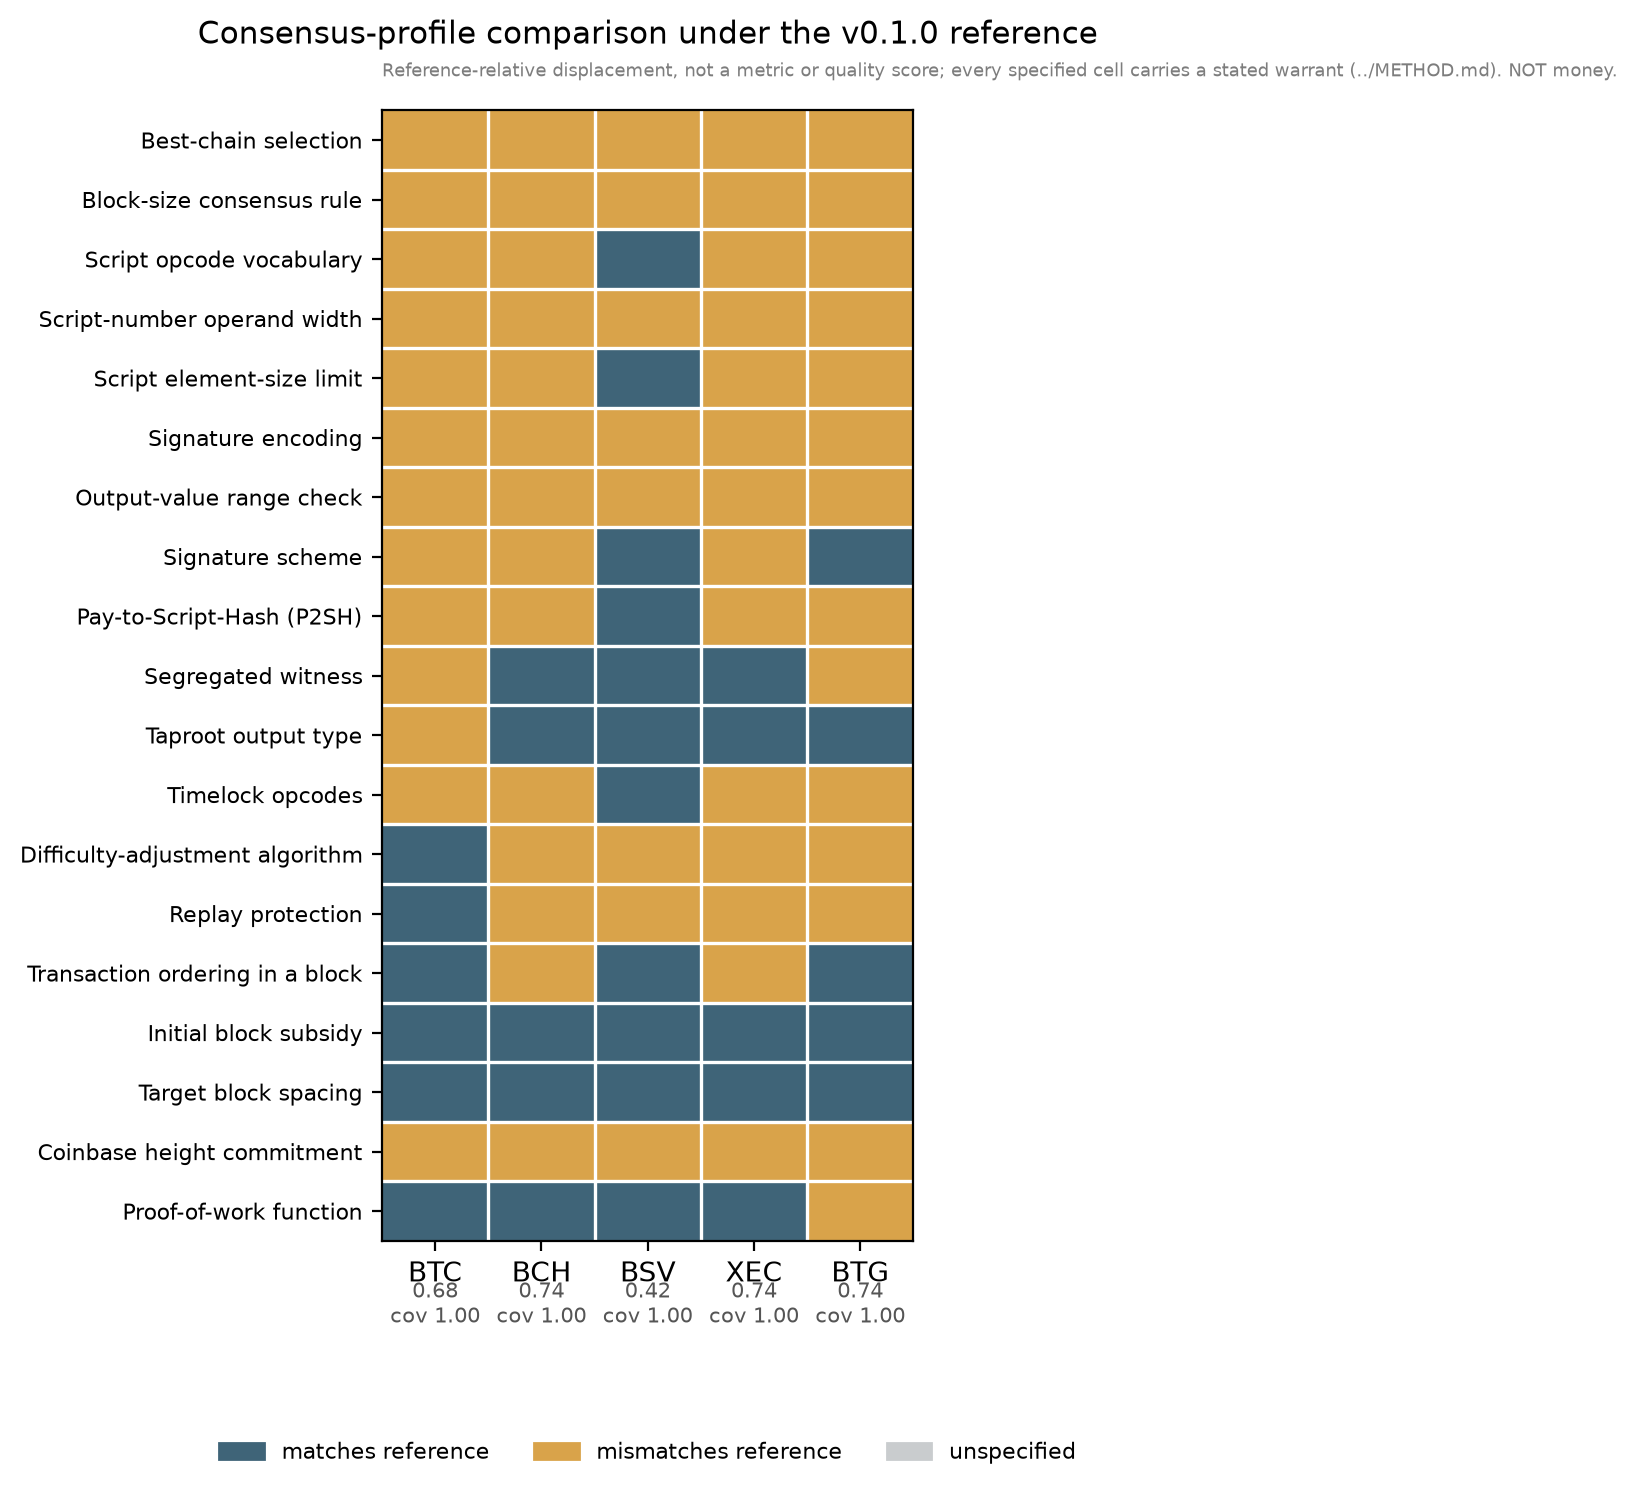
\includegraphics[width=0.9\linewidth,height=\textheight,keepaspectratio,alt={Axis-level agreement with the v0.1.0 reference. Each row is one of the 19 consensus axes and each column one chain. Every cell is filled; the colour, not the fill, carries the meaning --- one shade marks a value differing from v0.1.0 and the other a value matching it. Regenerated by figures/mismatch\_heatmap.py from the same engine that produces the tables.}]{figures/mismatch_heatmap_v010.png}
\caption{Axis-level agreement with the v0.1.0 reference. Each row is one
of the 19 consensus axes and each column one chain. \textbf{Every cell
is filled; the colour, not the fill, carries the meaning} --- one shade
marks a value differing from v0.1.0 and the other a value matching it.
Regenerated by \protect\texttt{figures/mismatch\_heatmap.py} from the
same engine that produces the tables.}
\end{figure}

\subsection{4.1 Decomposing agreement with v0.1.0: retention and
restoration}\label{decomposing-agreement-with-v0.1.0-retention-and-restoration}

A chain can agree with the reference for two very different reasons: it
did not change the rule (\textbf{retention}), or it adopted a change and
later removed it (\textbf{restoration}). A bare mismatch rate cannot
tell these apart, and the distinction is one of the two parts of the
caution this method must carry (Section 5.1 measures the other, the
labelling). We therefore report it as a count.

\begin{longtable}[]{@{}lrrr@{}}
\caption{Decomposition of each chain's agreement with v0.1.0. A match
counts as a \emph{restoration} only where the chain demonstrably
\textbf{held a different value and later removed it}, with the
introducing and removing change both named; every other match is a
retention. Every chain's matches include the 2 constant axes on which
all profiles agree (initial block subsidy, target block spacing),
counted as retentions.}\tabularnewline
\toprule\noalign{}
chain & matches & retentions & restorations \\
\midrule\noalign{}
\endfirsthead
\toprule\noalign{}
chain & matches & retentions & restorations \\
\midrule\noalign{}
\endhead
\bottomrule\noalign{}
\endlastfoot
BTC & 6 & 6 & 0 \\
BCH & 5 & 5 & 0 \\
BSV & 11 & 7 & 4 \\
XEC & 5 & 5 & 0 \\
BTG & 5 & 5 & 0 \\
\end{longtable}

\textbf{BSV is the only chain in the set with any restorations at all},
and it has four: the script opcode vocabulary and the element-size limit
(both restricted by the August 2010 commit and re-enabled by the 2020
``Genesis'' upgrade \citep{bsv_genesis}); P2SH (a consensus rule on its
lineage from 2012, removed by Genesis); and the \textbf{timelock
opcodes} --- CLTV and CSV reached its lineage through BIP65 and BIP112
in 2015--16 and Genesis sunsets them, the specification stating that the
operations \emph{revert to NOPs, which have no effect}, which is
v0.1.0's value. \textbf{Its other 7 agreements --- including the absence
of segwit, Taproot and CTOR --- are retentions: BSV forked from Bitcoin
Cash in November 2018 and has not held any of them.}

\(\Rightarrow\) The caution is therefore more specific than a bare
mismatch rate suggests: \textbf{4 of BSV's 11 agreements are
restorations: axes on which the chain diverged from v0.1.0 and later
returned to the reference value.} A low mismatch rate can arise from
removing later additions as readily as from preserving original ones,
and it is not a verdict of authenticity, continuity, or intent.

\begin{quote}
\textbf{A note on how this table was arrived at, because it bears on the
method.} An earlier version of this analysis inferred restoration from
\emph{which source a cell cites}, on the reasoning that a cell citing a
chain's own upgrade specification marks a rule that chain legislated.
\textbf{That inference is false and the numbers it produced were wrong}
--- it reported BSV at 7 restorations and gave BCH and XEC two apiece. A
citation records where a value is \emph{documented}, not what the chain
previously did: BCH forked three weeks before segwit activated and so
did not have segwit to remove, yet its segwit cell cites the fork
specification. \textbf{The table is now an explicit list in which every
restoration names the change that introduced the rule and the change
that removed it}, and nothing is inferred. \emph{A citation is not a
history.}
\end{quote}

\subsection{4.2 The references do not agree with each
other}\label{the-references-do-not-agree-with-each-other}

The engine compares references to chains. Asking it to compare the
references \emph{to each other} yields the result we consider most
important in the paper:

\begin{longtable}[]{@{}lrrl@{}}
\caption{Reference-against-reference disagreement. Every pair of
candidate origins, over the axes both specify. \textbf{They partly agree
and partly disagree} --- the whitepaper and the November pre-release
share no axis at all; the November pre-release and v0.1.0 share 3 and
differ on 2 --- so the choice of reference is not a technical
preliminary to the question but the substance of it.}\tabularnewline
\toprule\noalign{}
pair & jointly specified & differing & axes \\
\midrule\noalign{}
\endfirsthead
\toprule\noalign{}
pair & jointly specified & differing & axes \\
\midrule\noalign{}
\endhead
\bottomrule\noalign{}
\endlastfoot
whitepaper vs nov08 & 0 & 0 & \emph{(no overlap -- undefined)} \\
whitepaper vs v0.1.0 & 1 & 1 & fork\_choice \\
nov08 vs v0.1.0 & 3 & 2 & subsidy\_base, block\_spacing \\
\end{longtable}

\textbf{The single consensus axis the whitepaper specifies is one the
released client does not implement as described.} The paper describes
best-chain selection by accumulated proof-of-work; the January 2009
client selects by height. \textbf{Of the 3 axes the November pre-release
shares with v0.1.0, 2 differ and one agrees} --- the subsidy and the
block spacing changed between the preview and the release; the
proof-of-work function did not.

\(\Rightarrow\) \textbf{``The origin'' is not one object.} Displacement
is measured from whichever origin is chosen, and the available origins
do not describe one ruleset: of the three pairs, one shares no axis at
all; one shares a single axis and differs on it; one shares 3 and
differs on 2. This is the strongest available argument for the paper's
own insistence that its output is \emph{reference-relative}, and we
would rather state it than have a reader discover it.

\section{5. Robustness}\label{robustness}

\textbf{Leave-one-axis-out.} The v0.1.0 mismatch rates stay within BSV
{[}0.3889, 0.4444{]}, BTC {[}0.6667, 0.7222{]}, and BCH, XEC and BTG
{[}0.7222, 0.7778{]}; no single axis drives the ordering.

\textbf{Dropping up to three axes --- and why this is weaker than it
looks.} Over all 1160 subsets obtained by dropping up to three of the 19
axes the ranges are BSV {[}0.3125, 0.5000{]}, BTC {[}0.6250, 0.8125{]},
and BCH, XEC and BTG {[}0.6875, 0.8750{]}, and the lowest-mismatch chain
is BSV in 1160 of 1160. \textbf{But that is arithmetic, not a finding.}
All five chains share the denominator 19, so the mismatch \emph{counts}
(8, 13, 14, 14, 14) order the rates, and the gap from BSV to the
runner-up is 5. Dropping \(k\) axes moves any count by at most \(k\), so
the ordering \emph{cannot} change for \(k<5\): invariance up to 4
dropped axes is a theorem. Exhaustively, the first ties appear at
\(k=5\) (21 of 11628 subsets) and the first strict reversal at \(k=6\)
(7 of 27132). \textbf{We report this because a referee found it, and
because a robustness claim that is secretly a tautology is worse than
none at all.}

\textbf{Individuation.} Collapsing segwit, Taproot and Schnorr into one
axis moves every chain, and we report all five rather than the two that
suit the argument:

\begin{longtable}[]{@{}lrrr@{}}
\caption{Merged individuation. The post-2017 witness and
signature-scheme axes are collapsed into a single axis, and every rate
recomputed. \textbf{Every chain moves, and they do not move in the same
direction} --- which is the point: individuation is not a neutral
bookkeeping choice.}\tabularnewline
\toprule\noalign{}
chain & base & merged & change \\
\midrule\noalign{}
\endfirsthead
\toprule\noalign{}
chain & base & merged & change \\
\midrule\noalign{}
\endhead
\bottomrule\noalign{}
\endlastfoot
BTC & 0.6842 (13/19) & 0.6471 & -0.0372 \\
BCH & 0.7368 (14/19) & 0.8235 & +0.0867 \\
BSV & 0.4211 (8/19) & 0.4706 & +0.0495 \\
XEC & 0.7368 (14/19) & 0.8235 & +0.0867 \\
BTG & 0.7368 (14/19) & 0.8235 & +0.0867 \\
\end{longtable}

\emph{(Rates are given to four places, with the exact fraction beside
the base rate. \texttt{0.625} and \texttt{0.8125} are exact binary
values on a rounding tie, and two-place rounding of them is
convention-dependent --- an earlier draft printed \texttt{0.63}, which
is not a number the engine emits under any rounding mode.)} An earlier
draft described this cluster as ``BTC-only'' and reported only BTC and
BSV. That was wrong in both respects: Schnorr is a divergence for BCH
and XEC as well, and \textbf{the merge moves those two chains further
than it moves BTC}. The merge moves \textbf{every} chain and not in one
direction: BTC -0.0372, BSV +0.0495, and BCH, XEC and BTG +0.0867 each
--- reported in full rather than for the two that suit the argument. BSV
remains lowest under the merged individuation.

\textbf{Confidence.} The 7 medium-confidence cells (script-limit,
signature-scheme and timelock details on BCH, BSV and XEC) lie inside
all of these ranges and do not change the ordering.
\textbf{Exhaustively, and now computed rather than asserted:
\texttt{confidence\_sensitivity()} enumerates all 128 assignments of
those cells to match or mismatch, and BSV is uniquely lowest in 128 of
them.} This result was previously stated in the text and produced by no
code; it is emitted to \texttt{tables/figures.json} so that it follows a
cell edit instead of outliving one.

\subsection{5.1 Label granularity --- the sensitivity of the encoding
itself}\label{label-granularity-the-sensitivity-of-the-encoding-itself}

Two profiles match iff their labels are \textbf{equal as strings}. The
choice of label is therefore itself a coding decision, and the shipped
dataset contains a case where two labels name the same condition:

\begin{verbatim}
v0.1.0  block_size_rule = "no-dedicated-cap"
BSV     block_size_rule = "no-consensus-cap"
\end{verbatim}

Both mean \emph{no consensus rule caps the block size}. \textbf{Scored
as a mismatch purely because the strings differ.} The same applies to
\texttt{unbounded-openssl} versus \texttt{unbounded} on script-number
width. Conversely, a coder could reasonably argue the opposite way on
\texttt{script\_opcodes}: BSV's post-Genesis vocabulary is not v0.1's,
since it adds \texttt{OP\_CHECKDATASIG}, \texttt{OP\_SPLIT} and
\texttt{NUM2BIN}/\texttt{BIN2NUM} while still disabling
\texttt{OP\_2MUL}, \texttt{OP\_2DIV}, \texttt{OP\_VERIF} and
\texttt{OP\_VERNOTIF}.

\begin{longtable}[]{@{}
  >{\raggedright\arraybackslash}p{(\linewidth - 10\tabcolsep) * \real{0.1667}}
  >{\raggedleft\arraybackslash}p{(\linewidth - 10\tabcolsep) * \real{0.1667}}
  >{\raggedleft\arraybackslash}p{(\linewidth - 10\tabcolsep) * \real{0.1667}}
  >{\raggedleft\arraybackslash}p{(\linewidth - 10\tabcolsep) * \real{0.1667}}
  >{\raggedleft\arraybackslash}p{(\linewidth - 10\tabcolsep) * \real{0.1667}}
  >{\raggedleft\arraybackslash}p{(\linewidth - 10\tabcolsep) * \real{0.1667}}@{}}
\caption{Label granularity. Each row re-scores the whole comparison
under one defensible alternative \emph{labelling} of states that are
already agreed as facts. \textbf{Only BSV moves.} Relabelling shifts it
0.0526 from its base rate against 0.0322 for removing any single axis
--- \textbf{one cell's individuation can matter more than an entire
axis} --- though dropping up to three axes moves it further still,
0.1086.}\tabularnewline
\toprule\noalign{}
\begin{minipage}[b]{\linewidth}\raggedright
relabelling
\end{minipage} & \begin{minipage}[b]{\linewidth}\raggedleft
BTC
\end{minipage} & \begin{minipage}[b]{\linewidth}\raggedleft
BCH
\end{minipage} & \begin{minipage}[b]{\linewidth}\raggedleft
BSV
\end{minipage} & \begin{minipage}[b]{\linewidth}\raggedleft
XEC
\end{minipage} & \begin{minipage}[b]{\linewidth}\raggedleft
BTG
\end{minipage} \\
\midrule\noalign{}
\endfirsthead
\toprule\noalign{}
\begin{minipage}[b]{\linewidth}\raggedright
relabelling
\end{minipage} & \begin{minipage}[b]{\linewidth}\raggedleft
BTC
\end{minipage} & \begin{minipage}[b]{\linewidth}\raggedleft
BCH
\end{minipage} & \begin{minipage}[b]{\linewidth}\raggedleft
BSV
\end{minipage} & \begin{minipage}[b]{\linewidth}\raggedleft
XEC
\end{minipage} & \begin{minipage}[b]{\linewidth}\raggedleft
BTG
\end{minipage} \\
\midrule\noalign{}
\endhead
\bottomrule\noalign{}
\endlastfoot
as published & 0.6842 & 0.7368 & 0.4211 & 0.7368 & 0.7368 \\
block-size labels unified & 0.6842 & 0.7368 & 0.3684 & 0.7368 &
0.7368 \\
script-number qualifier dropped (inert since the BSV cell became
32mb-limit) & 0.6842 & 0.7368 & 0.4211 & 0.7368 & 0.7368 \\
BSV opcode set individuated & 0.6842 & 0.7368 & 0.4737 & 0.7368 &
0.7368 \\
the two unification cases together & 0.6842 & 0.7368 & 0.3684 & 0.7368 &
0.7368 \\
\end{longtable}

\begin{quote}
\mbox{}%
\subsubsection{\texorpdfstring{\(\Rightarrow\) BSV SPANS {[}0.3684,
0.4737{]} UNDER RELABELLING --- WIDER THAN LEAVE-ONE-OUT {[}0.3889,
0.4444{]}.}{\textbackslash Rightarrow BSV SPANS {[}0.3684, 0.4737{]} UNDER RELABELLING --- WIDER THAN LEAVE-ONE-OUT {[}0.3889, 0.4444{]}.}}\label{rightarrow-bsv-spans-0.3684-0.4737-under-relabelling-wider-than-leave-one-out-0.3889-0.4444.}

\textbf{None of these is a correction.} Each is a labelling a competent
coder could have chosen from the same primary sources. \textbf{The
spread is the result}, and it is the honest answer to what an earlier
draft of this paper claimed when it said there was \emph{``nothing for
two independent coders to disagree about''}. There is: they can disagree
about individuation, and that disagreement moves the score 0.0526 ---
more than removing any single axis does (0.0322), though less than
dropping up to three (0.1086).

\textbf{This does not weaken the instrument; it locates its soft joint.}
A displacement measure defined by label equality inherits every
judgement embedded in the labels. Reporting that explicitly is the
difference between a measurement and an assertion. \textbf{The soft
joint was identified in review, not in construction} --- which is itself
evidence about where a label-equality measure is weakest.
\end{quote}

\section{6. Interpretation}\label{interpretation}

The output is \textbf{reference-relative consensus-rule displacement},
nothing more. It is \emph{not a metric}, and the reason is stronger than
an earlier draft stated. That draft said identity-of-indiscernibles
fails because \emph{``distinct profiles can share a mismatch rate''} ---
but sharing a value is not a failure of that axiom. \textbf{The real
failure is that distinct profiles can sit at distance ZERO.} Take two
axes and profiles \(A=(0,\emptyset)\), \(B=(0,1)\), \(C=(1,1)\). Under
skip-unspecified \(d(A,B)=0\) although \(A \neq B\); and \(d(A,C)=1\)
while \(d(A,B)+d(B,C)=0+\tfrac{1}{2}\), so the triangle inequality fails
too. We therefore do not call it a metric. It is \emph{not a quality
score} and \emph{not a ranking of which chain ``is'' Bitcoin}: protocol
identity also involves naming, continuity, adoption, and governance,
none of which this instrument measures or should. What the instrument
does provide is a way to state --- and have anyone re-derive --- that,
on a fixed, source-anchored set of consensus axes, chain X's rules
differ from reference Y on a specific fraction of the jointly-specified
axes, with the sensitivity of that fraction made explicit.

\section{7. Limitations}\label{limitations}

\textbf{Granularity.} The axis enumeration, though rule-governed, still
embodies a choice of granularity; the four sensitivity analyses bound
but do not eliminate its influence. Relatedly, only 14 of the 19 axes
discriminate between chains at all (Section 2), so the reported rates
contain a fixed component that carries no comparative information.

\textbf{Coverage.} Coverage is intrinsically low for the two earlier
references, which limits what can be said against them --- a limit we
report rather than paper over, and which Section 4.2 shows to be more
than a technicality: \textbf{the only axis on which any two references
agree is the proof-of-work function, and they differ on every other axis
they share.}

\textbf{No historical evaluation.} Values are asserted at a single
frozen date, 1 August 2026. The engine accepts an \texttt{-\/-at}
argument and \textbf{refuses} any other date, earlier or later. It
previously accepted one and returned byte-identical output, because no
cell records when its rule activated; that silent no-op has been
replaced by an explicit refusal naming what is missing. Making the
instrument answer historically would require replacing each chain cell's
single value with a sourced timeline --- roughly 95 cells, each needing
the activation date its primary source states. That is real work, it is
not done, and we prefer to say so than to ship a flag that appears to do
it. \textbf{We note this because a paper whose claim is reproducibility
is exactly the paper in which an inert control is most damaging: a
reader who finds one has no way to judge which other capability is also
decorative.}

\textbf{A population that is eligible, not proven closed.} The
chain-selection criteria were fixed before application to the candidate
audit, and that audit applies them to candidates outside the set ---
which is how Bitcoin Gold was found to qualify and became a fifth
measured chain rather than a fourth criterion. \textbf{But passing that
test on a hand-built candidate list does not prove the list is
complete.} The criteria say which chains are \emph{eligible}; they do
not certify that every eligible descendant has been enumerated. We
therefore claim only that \textbf{these five qualifying chains were
identified by the candidate audit}, and not that they are every chain
the rule admits. This is the same posture as the axis set:
\textbf{admissible, not exhaustive} --- and both weakenings were forced
by external checks rather than found internally, which is itself the
honest thing to report about the method.

\textbf{Scope.} The method is deliberately confined to consensus rules;
it says nothing about the economic, social, or governance dimensions of
the chains it compares, and must not be read as if it did. It
generalises beyond Bitcoin to any protocol lineage with documented
change logs, which is its intended contribution.

\textbf{Source attribution, and what a census of it found.} The method's
premise is that a reader may contest any cell against its cited source,
which requires the citation to be the \emph{right} one. We therefore
audited the citations mechanically rather than asserting them:
\texttt{audit\_btc.py} fetches the BIPs repository and confirms
\textbf{8 of 8} BIP-backed BTC probes (over 7 cells; one cell is probed
through two BIPs), and \texttt{audit\_descendants.py} fetches the
Bitcoin SV, Bitcoin Cash and Bitcoin ABC primary specifications and
confirms \textbf{18 of 18} probes across BCH, BSV and XEC. Each fetch
carries a control requiring the document to name itself, so a challenge
or error page cannot be read as an answer. \textbf{The same script also
probes Bitcoin Gold's own \texttt{chainparams.cpp} for the 5 cells that
distinguish it, and confirms 5 of 5}, so all 5 are recorded in
\texttt{tables/audit\_descendants.json} alongside the others. \emph{(A
third script, \texttt{audit\_btg.py}, is not a citation audit at all: it
tests chain-selection criterion (2) --- whether Bitcoin Gold was
producing blocks at the freeze --- and it is why Bitcoin Gold is
measured here rather than excluded. It emits no citation ledger because
it verifies no cell.)} \textbf{Two units are in play here and they must
not be added across.} The non-BTG probes number 26 over 24 distinct
\emph{cells} --- a cell can be probed more than once: BTC's timelock
opcodes through BIP65 and BIP112, and BSV's script-number width through
two specifications. Adding Bitcoin Gold's 5 probes, none of which
repeats an earlier cell, gives \textbf{31 probes over 29 cells}. The
fetched figure quoted throughout this paper is the \emph{cell} count.
\textbf{The split is by chain, not by script}, because Bitcoin Gold's
cells were the ones added last.

\textbf{Three denominators appear in this paper and they are not
interchangeable:} \textbf{152} total profile cells, \textbf{118} of them
carrying a value across all profiles, and \textbf{95} specified cells on
the five \emph{chains} --- which is the denominator the audit partition
uses, because that partition is defined over the descendant-chain cells;
the three historical reference profiles are source-anchored separately
and are not part of it.

\textbf{Those are pass rates on the probes that were run, and a pass
rate is not a coverage figure.} The denominator matters more than the
numerator, so the engine partitions all 95 specified cells by \emph{what
each one's warrant actually is}:

\begin{longtable}[]{@{}
  >{\raggedright\arraybackslash}p{(\linewidth - 2\tabcolsep) * \real{0.5000}}
  >{\raggedleft\arraybackslash}p{(\linewidth - 2\tabcolsep) * \real{0.5000}}@{}}
\caption{Audit coverage, partitioned by what each cell's warrant
actually is. \textbf{A pass rate on the probes that were run is not a
coverage figure; this is the denominator.}}\tabularnewline
\toprule\noalign{}
\begin{minipage}[b]{\linewidth}\raggedright
warrant
\end{minipage} & \begin{minipage}[b]{\linewidth}\raggedleft
cells
\end{minipage} \\
\midrule\noalign{}
\endfirsthead
\toprule\noalign{}
\begin{minipage}[b]{\linewidth}\raggedright
warrant
\end{minipage} & \begin{minipage}[b]{\linewidth}\raggedleft
cells
\end{minipage} \\
\midrule\noalign{}
\endhead
\bottomrule\noalign{}
\endlastfoot
\textbf{fetched} -- a primary source retrieved and matched mechanically
& 29 \\
\textbf{inherited} -- argued from an ancestor pre-dating every fork in
the set & 51 \\
\textbf{absence} -- unconfirmable by construction & 9 \\
\textbf{unclassified} -- anchored to a cited source, not yet fetched &
6 \\
\textbf{total specified} & 95 \\
\end{longtable}

The unclassified group is the honest residue and it is not empty;
several of its cells are also the medium-confidence ones, which is why
the confidence sensitivity in Section 5 matters. \textbf{We state this
partition rather than the two pass rates alone, because the pass rates
read as a census and are not one.}

The census changed two citations and \textbf{no values}. BCH's
script-integer cell cited the May 2022 upgrade, which delivered 64-bit
integers; arbitrary precision arrived with CHIP-2024-07 BigInt,
activated 15 May 2025 --- still before the freeze, so the value stood
and only the source was wrong. BSV's signature-scheme cell cited the
Genesis specification, which contains no occurrence of \emph{ECDSA} or
\emph{Schnorr}; it is an absence, and is now cited and scored as one.
Separately, three attributions warrant a reader's attention without
being errors: strict-DER encoding on BCH, BSV and XEC is inherited from
BIP66 (2015) rather than originating at the 2017 fork, and BSV's CW-144
difficulty algorithm originates in the November 2017 Bitcoin Cash
upgrade rather than the August 2017 fork.

\textbf{Claims of absence are the dataset's weakest footing, and they
are structurally so.} The absence-warranted cells --- 9 of them:
\textbf{segwit on BCH, BSV and XEC} (Bitcoin Gold forked after segwit
activated and therefore has it), \textbf{Taproot on BCH, BSV, XEC and
BTG}, and \textbf{the Schnorr signature scheme on BSV and BTG} ---
cannot be confirmed by a fetch, because \textbf{no document establishes
that a rule was not adopted} and so no fetch can return a document
asserting the value: a specification can record a removal, as Bitcoin
SV's Genesis specification does for P2SH and the element-size limit, but
non-adoption leaves nothing to cite. They rest on chronology, a fork
cannot remove what it did not have, together with the absence of any
upgrade specification introducing them. This is weaker than a positive
citation, it is not remediable by searching for a record that
non-adoption does not produce, and it is reported here rather than left
for a reader to infer from the fact that the audit did not cover it.
\emph{The partition is by warrant, not by label. Of the 9, seven carry
the value \texttt{none} and the two Schnorr cells carry
\texttt{ecdsa-only}; three other chain cells carry \texttt{none} ---
BTC's replay protection, inherited from v0.1.0, and BSV's P2SH and
element-size limit, documented removals --- and are classified as
inherited or fetched accordingly, so Table 2 shows ten \texttt{none}
cells on the chains and the partition shows 9 absence cells.}

\section{8. Conclusion}\label{conclusion}

Situating chains against a historical reference need not be advocacy. By
making the axes explicit and freezing them before each reported run,
anchoring every value to a stated warrant --- a primary source for all
but the absence cells --- reporting coverage alongside mismatch, and
exposing sensitivity, the comparison becomes a computation a reader can
rerun and contest cell by cell --- reproducibility standing in for the
inter-rater machinery a subjective coding would need. The worked result
is itself instructive: the ``distance from the origin'' question is
degenerate against the whitepaper, low-coverage against the preview,
and, against v0.1.0, yields an ordering that is source-anchored yet
reference-relative and individuation-sensitive --- which is precisely
why it should be read as a measurement, not a verdict. Two of the
instrument's own outputs make that case better than the argument does.
The chain with the fewest mismatches is also the only one that reaches
\emph{any} of its agreement by removal rather than preservation --- 4
axes of 11, with the other 7 recorded as retentions --- and a
displacement measure is constitutionally unable to tell the two apart;
and the three candidate origins do not describe one ruleset --- of the
three pairs, one shares no axis at all; one shares a single axis and
differs on it; one shares 3 and differs on 2 --- so the choice of
reference is not a technical preliminary but the substance of the
question. \textbf{A measurement that discloses what it cannot see is
more useful than one that does not, and building the disclosure into the
engine keeps it in every rerun rather than in a footnote.}

\section{Data and Code Availability}\label{data-and-code-availability}

Every numerical result and table in this paper regenerates from
\texttt{obl\_metric.py}, and \texttt{figures/mismatch\_heatmap.py}
renders Figure 1 deterministically from the engine's axis-matrix output.
The engine carries the axis dataset it embeds. Running it writes
\texttt{comparison.json} (the full cell-level record, including the
criterion, cited source and confidence for each of the 152 cells, 34 of
which are unspecified), \texttt{comparison.csv} (the summary), and
\texttt{axis\_matrix.csv} (the raw axis values); the figure regenerates
from the same engine. \textbf{The replication package is archived on
Zenodo under the concept DOI
\url{https://doi.org/10.5281/zenodo.21964446}, which resolves to the
latest version --- 1.0.4 for this text, whose own version DOI is printed
in that record; version 1.0.0, deposited on 16 August 2026, remains at
\url{https://doi.org/10.5281/zenodo.21964447}} --- and the same
artifacts are in the repository at
\url{https://github.com/original-bitcoin-laboratory/genesis}, under
\texttt{paper-artifacts/obl-metric/} at the signed tag
\texttt{obl-metric-v1.0.4}. \emph{The DOI is the durable address; the
signed tag identifies the frozen repository version, and the commit it
resolves to is recorded in the Zenodo version record (a document cannot
carry the digest of the commit that contains it); the repository path is
a convenience that may move.} \textbf{Every reported rate, count and
coverage figure in this paper is interpolated from the engine's output
when the manuscript is built, not typed}, so the reported values are
re-derived on every build rather than compared against the engine as of
a date. The digests below identify the engine outputs from which the
reported results can be independently reconstructed.

\textbf{The bytes, not just the address.} A repository URL is a promise:
it can be edited after publication and a reader cannot tell. So the
scoring, audit and figure artifacts underlying every reported result
name themselves, by full SHA-256:

\begin{verbatim}
obl_metric.py
c57741458a459169e909aefdf5c1516e0460458c48d7c80d311770edd93752c2
audit_descendants.py
74daf47d77aa8266561963f8e4115eaa7376859450c1c9b923b8f94f40240214
audit_btc.py
daa7dcaebc464a206881be1107b463b510a61a86906d747012e7bc2013e01369
audit_btg.py
8de0a38b4e968662f2ea0e2d604a1c77a55ca2874bc54e5a381b2165679a5f65
figures/mismatch_heatmap.py
e5b3c633ef75ddd8171a8bb3036eb7201cddccfe883c8ee34cc4509fe6af71f6
figures/mismatch_heatmap_v010.png
d6ace5be32c6f94c7d78f36817bf93f0fdeed5af9e5ebee2af4af5b2f996b9de

tables/audit_descendants.json   run 2026-08-14T22:39:05+00:00
a35b7def457c9bda17d8c05edec334fb2aec827858cd6706c42569727c184ebc
tables/audit_btc.json           run 2026-08-14T22:38:41+00:00
ab63eef2f14674fcce02149a8d4d9136164706e551722bd535b2428d786f1efb

artifacts/comparison.json
2209d84e4cf03c7297016fec4cda05d23b00331ce3bc42601c5729801528bcc9
artifacts/axis_matrix.csv
191d70b5ee1206ec42e9184fbb5ce2624c99bd94788087b1f87a5c1f0175aaf2
artifacts/comparison.csv
71bb2fa5a06cf72a68ef6fa80578fc1eab3ed0d04da432518c675b46eb254e18

tables/table*.md   manifest over the 8 engine-emitted table files
11afe004a45e10c0fd655aff7767d47a41e6f02e1158fba3c55028a751a8f221
\end{verbatim}

Any copy that does not hash to these is not the copy this paper reports
on. \textbf{The two \texttt{tables/audit\_*.json} entries are the audit
ledgers, and they are what tie the reported audit figures to recorded
output rather than to source files that merely existed.} Each records
its own run timestamp and, per probe, the URL fetched, the HTTP status,
the control outcome and the SHA-256 of the retrieved body; the 31 probe
records over 29 distinct cells reported in Section 7 are the contents of
those two files --- Bitcoin Gold's 5 included, since
\texttt{audit\_descendants.py} performs them.

\emph{A digest change is therefore legible, within what a digest can
establish.} \textbf{If a ledger digest changes, the recorded audit
output changed, and the embedded run timestamp identifies the execution
that the ledger records. If only a script digest changes while its
ledger digest and run timestamp do not, the published audit output has
not been regenerated under those new script bytes.} \emph{A digest
proves which bytes exist, not how they came to exist: the timestamp is a
recorded claim about an execution, not proof that one occurred. The
narrower statement is the one the evidence supports.}

\textbf{The three \texttt{artifacts/} entries are the engine's principal
serialised outputs}, and they give the engine the counterpart the
ledgers give the audit scripts. \texttt{comparison.json} pins the full
cell-level comparison record, \texttt{axis\_matrix.csv} pins the
canonical axis matrix, and \texttt{comparison.csv} pins the summary
rates. Every numerical table in this paper is emitted by the same engine
run whose comparison state those files serialise.

\textbf{Their digests establish byte identity, not the semantic reason
for a change.} A changed digest means that artifact changed; a diff
identifies whether the change touched values, sources, confidence,
criteria or serialisation. \emph{\texttt{comparison.json} records
criteria, primary sources and confidence alongside values, so a
citation-only correction moves its digest while every number in this
paper stays the same --- this work has made exactly such corrections.}
Conversely, if the engine digest changes while these three remain
byte-identical, what is established is that the serialised comparison
state and summary outputs are unchanged.

\textbf{The final entry pins the remaining link between that state and a
printed table.} The manuscript's numerical tables are substituted from
files the engine emits, and the manifest is one SHA-256, computed by
\texttt{obl\_metric.py} over each emitted table's file name (as UTF-8
bytes) followed by the raw 32-byte SHA-256 of its contents, with no
separator, in sorted file-name order, so those 8 files are pinned
without adding 8 lines. \emph{One presentation artifact remains
deliberately outside the list: \texttt{tables/figures.json}, which
carries the scalar substitutions --- it is the file every digest above
is recorded in, so it cannot contain its own.
\texttt{revision\_check\_live.py} covers it the other way round, by
re-deriving each scalar the paper prints from the engine and failing on
any difference.}

\emph{A generation timestamp was deliberately not embedded, and the
distinction is the point: it would change the digest on every run and
convert ``the output changed'' into ``time passed'', destroying the
property the pairing exists to provide. The audit ledgers carry
timestamps because they record network fetches, which are not
reproducible --- the descendant ledger's run is stamped
2026-08-14T22:39:05+00:00, after the 1 August freeze it audits; these
record computations, which are.} \textbf{The writers disable platform
line-ending translation, so these digests are properties of the data
rather than of the machine that produced them.} \emph{The digests cover
those files only --- not the fetched upstream sources, whose own hashes
are recorded per-probe inside the ledgers, and not
\texttt{tables/figures.json}, which cannot be listed here because it is
the file these digests are recorded in.} Recording any chain's rule
after a future upgrade would be a one-cell edit carrying a new primary
source under a new evaluation freeze, after which the entire table, the
sensitivity analysis and the figure recompute for that date; the 1
August 2026 results are not edited in place. \textbf{Once the encoding
is fixed there is no manual scoring step: the artifact performs the
derivation deterministically}, and a reader who disagrees with a value
can contest it cell by cell against the cited source. \emph{That is not
a claim that no human judgement is present --- it is present in the
encoding, and Section 5.1 measures how much the result moves when a
defensible alternative labelling is substituted.}

\textbf{Scope statement.} The experimental chains and artifacts
associated with this work carry no monetary value: there is no premine,
no sale, no token, and no price. Nothing in this paper is financial
advice, and the instrument takes no position on whether any chain should
change anything. \textbf{The instrument compares five chains that do
carry a market price; it measures none of it, and a mismatch rate must
not be read as a statement about any of them as an asset.}


\bibliography{paper}

\end{document}
